
\section{Latent Discourse Marker Guided Reasoning Path in Text based Question Answering} \label{sec:3-2}

\subsection{Background}
Reading comprehension (RC) tasks have gained lots of attention from NLP research community during the past few years.  Two types of RC tasks are widely studied: the extractive question answering task \cite{DBLP:conf/emnlp/RajpurkarZLL16,DBLP:conf/acl/RajpurkarJL18}, and the  multiple-choice question answering task \cite{DBLP:conf/aaai/AydinYLLGD14,DBLP:conf/aaai/KhashabiKSR18}. Most of the current state-of-the-art methods use deep neural networks (DNN) based structures to tackle these two tasks and achieve practical performance on a variety of RC datasets. The most recent DNN based model BERT \cite{DBLP:journals/corr/abs-1810-04805} has even outperformed human's performance on the SQuAD dataset \cite{DBLP:conf/emnlp/RajpurkarZLL16}. 
\begin{figure}[ht]
\centering
	{\fontsize{9}{10}\selectfont
    \setlength{\tabcolsep}{0.6mm}
%    \hspace{-2mm}
    \begin{tabular}{|p{75mm}|}
    \hline
\textbf{Context: }\textit{\textcolor{red}{After}} inflation stopped, \textit{\textcolor{blue}{reheating }}occurred \textit{\textcolor{red}{until}} the universe obtained the temperatures required for the production of a quark-gluon plasma \textit{\textcolor{red}{as well as}} all other elementary particles. \\
\textbf{Question: }When did \textit{\textcolor{blue}{reheating}} stop?     \\
\textcolor{gray}{(reasoning step 1: focus on the context to the right of ``until'')}\\
\textbf{Context: }the universe obtained the temperatures required for the production of a quark-gluon plasma \textit{\textcolor{red}{as well as}} all other elementary particles. \\
\textcolor{gray}{(reasoning step 2: focus on the context to the left of ``as well as'')}\\
\textbf{Answer: }until the universe obtained the temperatures required for the production of a quark-gluon plasma \\
\hline
    \end{tabular}
    }
\caption{An Example in QAMR: The words in italics are discourse markers (in red) and question topic words (in blue). Reasoning steps are highlighted in gray. }
\label{fig:qa_example}
\end{figure}

Most existing deep learning models are either deep structures without internal steps, or with internal steps that do not justify comprehension. In other words, these models generate answers directly without giving human-understandable reasoning of the answer. Another disadvantage of the end-to-end DNN models is that the model is only valid for a specific domain of the training data, that is, the knowledge is not transferable to datasets in other domains. %Also, the knowledge are not explainable or interpretable as reasoning (by users). 
By contrast, humans can answer questions following reasoning steps which are reproducible and transferable.  

To address these issues, we introduce a novel deep reasoning model for RC tasks, by taking advantage of the discourse information in the context. The model design is inspired by the reading behavior of a well trained reader (``mature reader''). A human reader would not search for the answer by simply reading the entire document without any focus. Instead he will look for the answer based on question topics and discourse markers ( \emph{e.g.} ``however'' and ``because'')~\cite{assiri2011test,sungatullina2016metacognitive}. Question topics and discourse markers can help the reader quickly select the most relevant segments (pieces of text) to read, and skip those less relevant ones. Figure \ref{fig:qa_example} gives an example on how a ``mature reader'' finds an answer to a given question in a context paragraph. First, by reading the question, the reader notices the topic word ``reheating'' and the question type ``when-''. Then the reader searches for words that indicate \emph{time} from the given context, which could be ``after'' or ``until''. By analyzing the relationship between these time indicators and the target word ``reheating'', the reader focuses on the context after ``until''. Next, the reader splits the current focus by the connective ``as well as'' into two clauses, which are complementary to each other. Finally, the reader picks the text segment between ``until'' and ``as well as'' as the final answer. In this way, we define a reasoning path as a sequence of binary selections based on discourse markers. In the next section, we will show how to model such a reasoning path as latent variable using reinforcement learning.


\subsection{An Interpretable Discourse Guided Deep Reasoning Model}

We propose a deep reasoning model (DRM) with an architecture as shown in Figure \ref{fig:systemDiagram}. The model has three components: the state generation module (SGM) implemented with two convolutional neural networks; the reasoning generation module (RGM) implemented as deep reinforcement learning via an actor-critic algorithm; and a context selection operator (CSO) that shrinks the text context given a discourse marker and a direction (left=before; right=after).


\begin{figure}
\centering
\begin{minipage}{.45\textwidth}
 \centering
 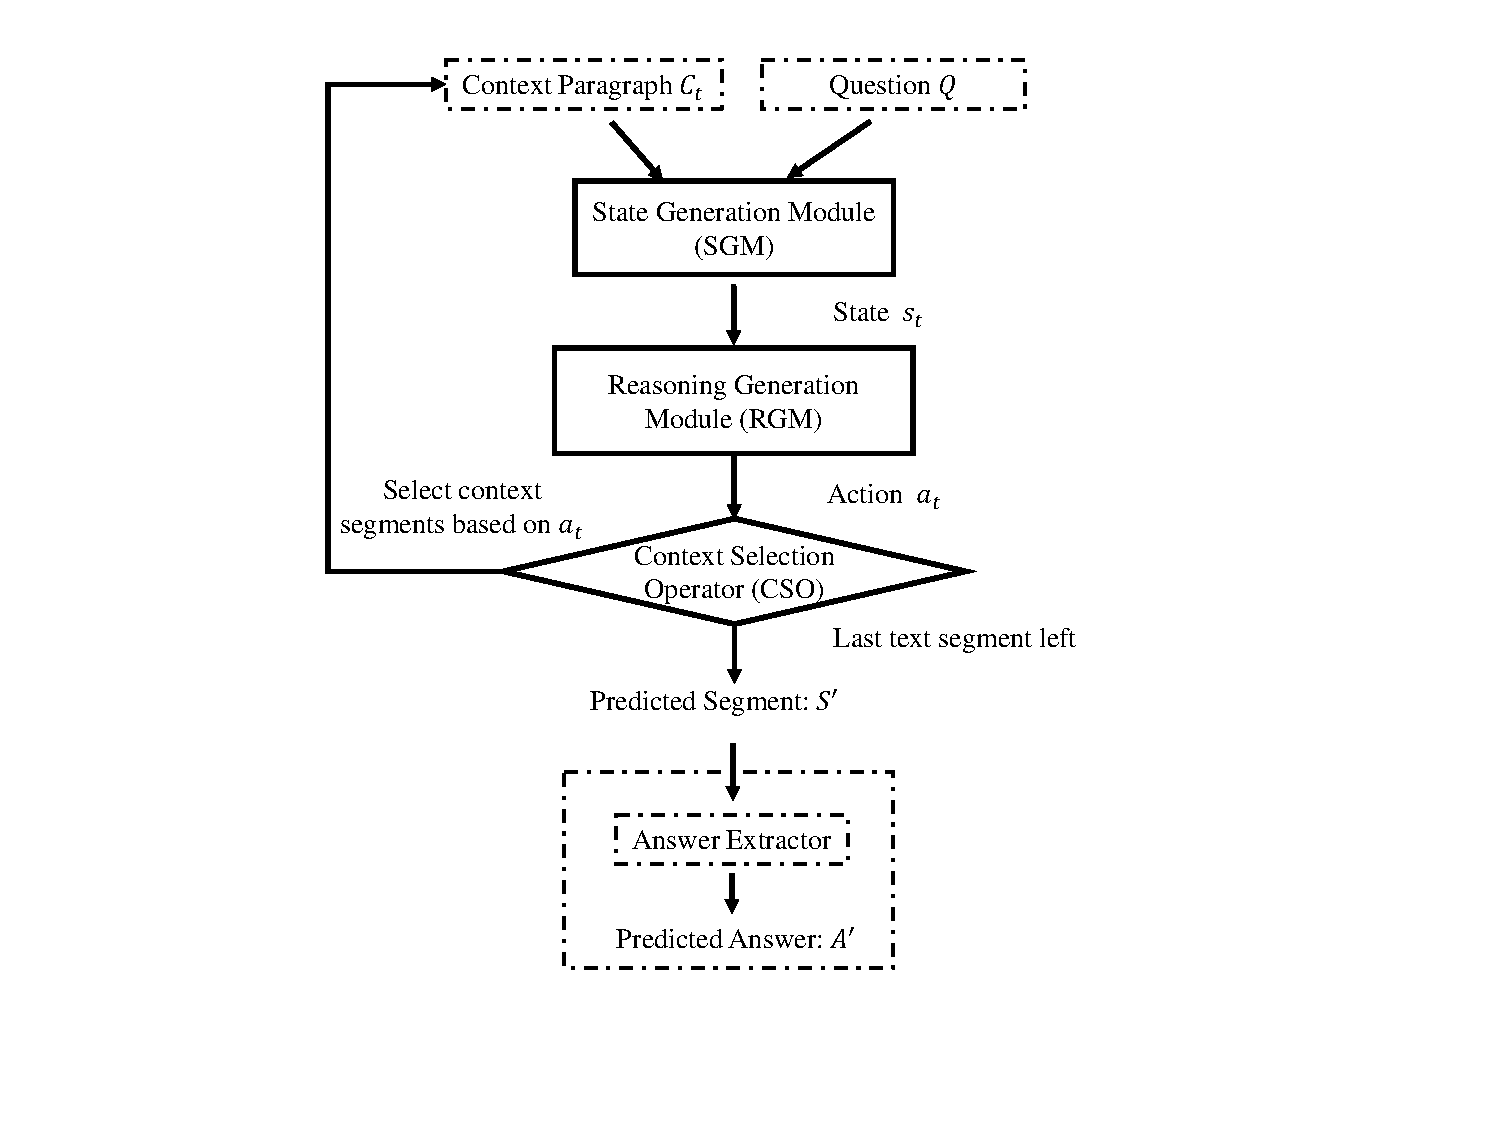
\includegraphics[width=0.9\linewidth]{Images/fig1.pdf}
 \caption{System Diagram}
 \label{fig:systemDiagram}
\end{minipage}
\end{figure}
%[Yu] \kechen{basic idea of RL and insight of using RL, multi step decision is naturally modeled by MDP}
% \subsection{Model Component Overview}
\label{sec2description}
The goal of our system is to mimic human reading behavior to extract a segment that
contains the answer. The mechanic in reducing the text context is analogous to binary search: Let $D=(D^1,D^2,...,D^k)$ be a list of discourse markers that appears in a context paragraph $C$. These discourse markers, working as the candidate partition points, divide the context into a list of segments $S=(S^1,S^2,...,S^{k+1})$. Then the context can be represented by a mixture of discourse markers and segments, $C=(S^1, D^1, S^2, D^2,...,D^k, S^{k+1})$. To identify the correct segment $S^*$ from $S$, our model at time-step $t$ works as follows:\\
(a) SGM encodes the context $C_t$ and question $Q$ into a vector representation, \emph{i.e.} the state $s_t$.\\
(b) RGM takes the state $s_t$ as its input, and predicts the partition point $D^{p(s_t)}_t$ (${p(s_t)}$ is the index selected at \emph{t}) and the reading focus $f_t \in \{left, right\}$. An action is defined as $a_t=(D^{p(s_t)}_t,f_t)$. \\
(c) CSO divides $C_t$ into two parts from $D^{p(s_t)}_t$: $C^1_t=(S^1, D^1,...,D^{p(s_t)-1}, S^{p(s_t)})$ and $C^2_t=(S^{p(s_t)+1}, D^{p(s_t)+1},...,D^k, S^{k+1})$, and keeps $C_{t+1} \leftarrow C_{t}^{1}$ if $f_t$ is left or $C_{t+1} \leftarrow C_{t}^{2}$ if $f_t$ is right. \\
The iterations stop when the output only contains a single text segment enclosed by two neighbor discourse markers. Intermediate output $D^{p(s_t)}_t$ at each time-step constitutes a reasoning path $(D^{p(1)}_1,...,D^{p(s_t)}_t)$. We note that during the prediction procedure the context $C_t$ changes, while the question $Q$ not (see Algorithm \ref{segment_alg}).

% \emph{Remarks:}
It is possible to add an answer extractor following the text segment $S'$ for a final answer (dashed in Figure \ref{fig:systemDiagram}). Since this is not our paper's focus and many existing works have been done achieve decent performance \cite{DBLP:conf/ijcai/HuPHQW018}, so this module is not discussed here. %\cite{DBLP:conf/acl/WangYWCZ17,DBLP:journals/corr/abs-1804-09541,DBLP:conf/ijcai/HuPHQW018}. Since this is not our paper's focus, we do not discuss it here.\\


%Since our paper's focus is not on answer extraction, and many existing works have been done achieve decent performance \cite{DBLP:conf/acl/WangYWCZ17,DBLP:journals/corr/abs-1804-09541,DBLP:conf/ijcai/HuPHQW018}, so this module is not discussed in this paper.



\begin{algorithm}
  \SetKwInOut{Input}{Input}
  \SetKwInOut{Output}{Output}

 % \underline{function Euclid} $(a,b)$\;
  \Input{$C$: context, $Q$: question}
  \Output{Answer segment: a single text segment enclosed by two neighbor discourse markers}
  $t = 0$\\
  $C_0 \leftarrow C$\\
  % Initialize model parameters\\
  \While {$C_t$ contains more than one text segment}{
    %SGM encodes the context $C_t$ and question $Q$ into a vector representation $s_t$.\\
    $s_t = SGM(C_t, Q)$ // generate state\\
    $D^{p(s_t)}_t,f_t= RGM(s_t)$ // generate action\\ 
   % $a_t=(D^{p(s_t)}_t,f_t)$ // an action consists of partition point $D^{p(s_t)}$ and reading focus $f_t$\\
    $C^1_t, C^2_t = CSO(C_t, D^{p(s_t)}_t)$\\
    \uIf{$f_t==left$}{
    //$C^1_t=(S^1, D^1,...,D^{p(s_t)-1}, S^{p(s_t)})$\\
        $C_{t+1} \leftarrow C_{t}^{1}$ 
    }\Else{
    //$C^2_t=(S^{p(s_t)+1}, D^{p(s_t)+1},...,D^k, S^{k+1})$\\
        $C_{t+1} \leftarrow C_{t}^{2}$ 
    }
    $t = t + 1$
  }
  $S^* \leftarrow C_t$\\
  \Return{$S^*$}
  \caption{Identifying the correct answer segment from the context}
  \label{segment_alg}
\end{algorithm}

We leverage a deep reinforcement learning (DRL) based structure to implement the reasoning generation module introduced in the above section. 
For every given context-question pair, the dataset provides an answer. Although this answer can be used to evaluate the final output of any reasoning path, there is no ground truth to evaluate the performance of each intermediate reasoning step $D^{p(s_t)}_t$. There are usually several different reasoning paths leading to the correct answer segment, based on different sequences of selecting discourse markers; thus the  task of searching for the best path fits well into the reinforcement learning, as these actions can reasonably imitate the human actions.

\begin{table*}[t]

	\begin{center}
	\resizebox{1.0\columnwidth}{!}{%resize the table
		\begin{tabular}{|l|c|c|c|c|cccccccc|}
			\hline
       \textbf{Method} & \textbf{Loss} & \textbf{Discourse} & \textbf{Target Word} 
      & \textbf{All} & \textbf{What} & \textbf{Whose} & \textbf{How} & \textbf{Why} & \textbf{Where} & \textbf{Who} & \textbf{When} & \textbf{Which} \\

            \hline
      Gradient Boosting & binary & &
      & .488 & .485 & .523 & .502 & .461 & .477 & .471 & .517 & .561 \\
      Gradient Boosting & binary & \checkmark &\checkmark 
      & .673 & .676 & .633 & .664 & .538 & .659 & .662 & .721 & .684 \\
            Gradient Boosting & ranking & & 
      & .469 & .486 & .397 & .414 & .566 & .475 & .447 & .453 & .457 \\
      Gradient Boosting & ranking & \checkmark &\checkmark 
      & .670 & .673 & .638 & .657 & .538 & .657 & .662 & .721 & .684 \\
      BM25 & ranking & &
      & .536 & .545 & .679 & .543 & .160 & .529 & .510 & .464 & .594 \\

      Coarse-to-Fine Answer Selector & binary & &
      & .540 & .539 & .490 & .506 & \textbf{.615} & .524 & .552 & .571 & .558 \\
     % CNN & binary & &
     % & .511 & .508 & .528 & .515 & .564 & .496 & .513 & .517 & .522 \\
      RaSoR & multi-class & &
      & .615 & .620 & \textbf{.706} & .598 & .560 & .599 & .598 & .586 & .659 \\
      \hline
      DRM-noRL & binary & \checkmark & \checkmark 
       & .664 & .667 & .619 & .649 & .564 & .653 & .657 & .706 & .678 \\
      DRM-type 1 & RL & \checkmark & 
      & .691 & .696 & .676 & .681 & \textbf{.615} & .696 & .671 & .724 & .702 \\
      DRM-type 2 & RL & \checkmark & \checkmark 
      & \textbf{.702}  & \textbf{.703} & .676 & \textbf{.684} & \textbf{.615} & \textbf{.701} & \textbf{.677} & \textbf{.733} & \textbf{.705} \\
      DRM-type 2 w/ human & RL & \checkmark & \checkmark 
      & \textbf{.797} & \textbf{.801} & \textbf{.789} & \textbf{.769} & \textbf{.820} & \textbf{.778} & \textbf{.793} & \textbf{.815} & \textbf{.810} \\
      \hline

		\end{tabular}

				}\vspace{0.4mm}	\\
\small{Table 3(a): Results on QAMR-SUBSET dataset.}\\\vspace{2mm}
	\resizebox{1.0\columnwidth}{!}{%resize the table
		\begin{tabular}{|l|c|c|c|c|cccccccc|}
			\hline
       \textbf{Method} & \textbf{Loss} & \textbf{Discourse} & \textbf{Target Word} 
      & \textbf{All} & \textbf{What} & \textbf{Whose} & \textbf{How} & \textbf{Why} & \textbf{Where} & \textbf{Who} & \textbf{When} & \textbf{Which} \\

            \hline
      Gradient Boosting & binary & &
      & .338 & .355 & .363 & .289 & .166 & .291 & .311 & .263 & .428 \\
      Gradient Boosting & binary & \checkmark &\checkmark 
      & .575 & .586 & .528 & \textbf{.616} & .666 & .632 & \textbf{.621} & \textbf{.610} & \textbf{.528} \\
            Gradient Boosting & ranking & & 
      & .360 & .376 & .454 & .339 & .666 & .354 & .335 & .276 & .301 \\
      Gradient Boosting & ranking & \checkmark &\checkmark 
      & .561 & .567 & .424 & .578 & .166 & .583 & .566 & .539 & .507 \\
      BM25 & ranking & &
      & .456 & .481 & .380 & .393 & .0.0 & .448 & .439 & .444 & .491 \\

      Coarse-to-Fine Answer Selector & binary & &
      & .405 & .422 & .363 & .408 & .166 & .312 & .376 & .315 & .492 \\
      %CNN & binary & &
      %& .356 & .346 & .242 & .359 & .666 & .437 & .376 & .355 & .365 \\
      RaSoR & multi-class & &
      & .539 & .545 & \textbf{.619} & .525 & .375 & .528 & .552 & .487 & .491 \\
      \hline
      DRM-noRL & binary & \checkmark & \checkmark 
       & .573 & .571 & .606 & .591 & .833 & \textbf{.645} & .572 & .513 & .539 \\
      DRM-type 1 & RL & \checkmark & 
      & .569 & .579 & .515 & .572 & \textbf{.833} & .625 & .560 & .513 & .492 \\
      DRM-type 2 & RL & \checkmark & \checkmark 
      & \textbf{.599} & \textbf{.599} & .575 & \textbf{.616} & \textbf{.833} & \textbf{.666} & .598 & .565 & .523 \\
      DRM-type 2 w/ human & RL & \checkmark & \checkmark 
      & \textbf{.676} & \textbf{.676} & \textbf{.727} & \textbf{.683} & \textbf{1.0} & .500 & \textbf{.698} & \textbf{.618} & \textbf{.682} \\
      \hline
    
		\end{tabular}

		}\vspace{0.4mm}	\\

	\end{center}
	\caption{Comparison of different approaches. We show the training loss (binary: binary cross entropy loss, ranking: ranking loss, multi-class: cross entropy loss, RL: reinforcement learning loss in formula \ref{rlloss}.), and check whether discourse or target word is used in each method. We highlight the top scores of each column in bold. 
  }\label{tab:main3}
\end{table*}

A typical reinforcement learning structure contains four main elements: the state ($s_t$), the action ($a_t$), the reward ($r_t$), and the policy ($\pi$). In general, by taking an action $a_t$, a RL agent can move from its current state $s_t$ to another state $s_{t+1}$ and receive a reward $r_t$. The final target of a RL model is to learn an optimal policy $\pi$ such that the system can maximize the expected total reward $R_t=\mathop{\mathbb{E}}_\pi[\sum_{t=0}^{T}\gamma^t r_t]$ obtained at each state $s_t$, where $s_T$ is the final state. Specifically in our problem, at each time-step $t$ our model is in state $s_t$ containing the information of the current context $C_t$ and the question $Q$; it takes action $a_t$ choosing the appropriate discourse marker and the direction (reading focus) in order to maximize the expected reward $R_t$. We consider two types of actions with/without using labeled question topic, and name them DRM-type 1 and DRM-type 2. More details of the RL configurations can be found in appendix \ref{sec:design}.

This study uses two corpora from Question-Answer Meaning Representations datasets \cite{DBLP:conf/naacl/MichaelSHDZ18}: the QAMR corpus and the PTB corpus. The QAMR corpus consists of 69,320 QA pairs for 4,238 context paragraphs extracted from Wikipedia, and the PTB corpus consists of 27,082 QA pairs for 253 context paragraphs extracted from Penn Treebank \cite{DBLP:journals/coling/MarcusSM94}. A target word, which appears in the question and represent the question topic is associated with each QA pair in the datasets. We report the overall segment prediction accuracy on the datasets and the accuracy on each question type (Table~\ref{tab:main3}). Descriptions of baseline methods can be found in appendix \ref{qa_baseline}. On both QAMR dataset and PTB dataset, DRM-type 2 with human in the loop achieves the highest accuracy. Being able to interact with humans is an advantage of our approach; 
% Humans can understand the decision process of the algorithm and can intervene if necessary. By contrast, 
none of the competitor approaches can do this, either because their decision process is a single-step process or because their decision process is not interpretable. In our experiment, 65\% QA pairs (less than the threshold) get help from human at one reasoning step, and their performance increases 0.15. It is also very interesting to learn that the remaining 35\% data points with high confidence reasoning learned by our model perform 0.06 better than the average performance. To further understand whether the improvement comes from human's selection or from our model's judgement, we allow the model to randomly select 65\% of the QA pairs, and for each pair, to interact with human once without considering their confidence. The results show that such random selection procedure doesn't make any difference on performance. Even without human's help, our DRM-type 2 model still achieves better performance than all other methods. As expected, DRM-type 2 model performs better than DRM-type 1 model, since type 2 actions leverage more information. 
%Looking at how the algorithm performs as the number of reasoning steps increases, the prediction accuracy increases slightly as the reasoning gets longer: the accuracy for 1-step, 2-step, 3-step and 4-step reasoning is 0.700,0.700,0.705 and 0.727.

Among the baseline methods, Gradient Boosting trained on both bag-of-words + discourse features works best. These models perform much worse if trained only on bag-of-words features. This shows that the structure/order information captured by discourse features is essential, which Neural network doesn't do. 
% The classical BM25 works well on questions that start with ``whose" but terribly on questions that start with ``why". 
Since BM25 solely relies on similarity between the question and the segment, it only works well when the the question and the correct segment have many overlapping words, as in the case of ``whose'' questions, but not ``why'' questions.

%0. RL learning curve\\




\begin{table*}[t]
\centering
{
	\fontsize{9}{9}\selectfont
  %\setlength{\baselineskip}{0pt}
  \setlength{\tabcolsep}{1.0mm}
  \renewcommand{\arraystretch}{1.1}
	%\hspace{4mm}
	\begin{tabular}{|p{1.8cm}|p{2.5cm}|p{2.5cm}|p{2.5cm}|p{5.8cm}|}
 	\hline
 	\textbf{Question genre}  & \textbf{Same side}& \textbf{Opposite sides}& \textbf{Context-dependent (side)} &  \textbf{Example QA pairs} \\
 	\hline
 	when \newline what year \newline how long 
 	& \textbf{step 1}: already, again, still, following \newline\textbf{step 2}: while, yet & \textbf{step 1}: as soon as, at that \newline\newline \textbf{step 2}: then, further, originally
 	&\textbf{step 1}: previously, until, back, after, soon, during \newline \textbf{step 2}: since, second, next, when, as well, because, who 
	&  \textbf{Context: }28 \textit{\textcolor{blue}{skiers}} earned DNFs \textit{\textcolor{red}{during}} \underline{the first run}, \textit{\textcolor{red}{and}} nine earned DNFs \textit{\textcolor{red}{during}} their second runs.
  \newline \textbf{Question: }When did \textit{\textcolor{blue}{skiers}} earn DNFs? 
  \newline \textbf{Learned Reasoning: } during-right, and-left\\ 
	\hline
  why \newline what caused 
 &\textbf{step 1}: in order to, because, due to,  since \newline\textbf{step 2}: as, but &\textbf{step 1}: at that, previously, though, if, since \newline \textbf{step 2}: second, for, to, or, that, not, and & \textbf{step 1}: well, following, initially  \newline\newline\textbf{step 2}: which, even,certainly  
  & \textbf{Context: }Given its initial condition, prediction of its final condition is possible, causally \textit{\textcolor{red}{but}} only probabilistically, \textit{\textcolor{red}{because}} the Schrödinger equation is deterministic for wave function evolution, \textit{\textcolor{red}{but}} \underline{the wave function describes the system only} \underline{\textit{\textcolor{blue}{probabilistically}}}.
  \newline \textbf{Question: }Why is the prediction \textit{\textcolor{blue}{probabilistic}}?
  \newline \textbf{Learned Reasoning: }because-right, but-right\\ 
	\hline	
	who+past tense 

	& \textbf{step 1}: rather, thus, including \newline\newline\textbf{step 2}: nor, who, initially &\textbf{step 1}: earlier, definitely, previously \newline\newline\textbf{step 2}: particularly, seemingly
		&\textbf{step 1}: ultimately, since, when, later, while, finally \newline \textbf{step 2}:  again, last, and , after, next, 
	& \textbf{Context: }\underline{Hatch had} \textit{\textcolor{red}{previously}} \textit{\textcolor{blue}{survived}} a separate crash in 2003, \textit{\textcolor{red}{that}} killed his mother, brother \textit{\textcolor{red}{and}} sister.
  \newline \textbf{Question: }Who \textit{\textcolor{blue}{survived}}?\newline \textbf{Learned Reasoning: }previously-left\\ 
	\hline
  where 
 
  
	 &\textbf{step 1}: following, to explain, while \newline\newline\textbf{step 2}: possibly, initially, finally, hence &\textbf{step 1}: to, before, back, in that, eventually \newline\textbf{step 2}: like, or, as & \textbf{step 1}: in which, then, second, next \newline\newline \textbf{step 2}: too, yet, second, including, after, next
  & \textbf{Context: }\textit{\textcolor{red}{Once}} the proposed \textit{\textcolor{blue}{amendment}} has passed those hurdles, \textit{\textcolor{red}{then}} the amendment goes \textit{\textcolor{red}{to}} \underline{Indiana voters} \textit{\textcolor{red}{who}} vote yea or nay on the amendment. 
  \newline \textbf{Question: }Where does the \textit{\textcolor{blue}{amendment}} go?
  \newline \textbf{Learned Reasoning: }to-right, who-left\\ 
 \hline
\end{tabular}
}
\caption{Top discourse markers are associated with question genres, and focus direction is learned in \textsc{QAMR-SUBSET} dataset. We show four different question genres: time, reason, person, and location.}
\label{tab:disc_phrase}
\end{table*}

\section{Proposed work}

In the question answering task, we have developed a QA system that attempts to generate both final answer and the interpretable reasoning path, then evaluated the performance of answer generation. A natural follow up work would be to evaluate the interpretability of the system. Since there is no direct way to evaluate reasoning chains, we propose to use human identification and run downstream tasks instead. 


\subsection{Evaluating with Human Identification} \label{future_reason}


We first propose to evaluate generated reasoning path with human identification. The goal is to inspect the trained model and find the discourse markers which have the greatest impact for each question type. In a preliminary study, we show a few samples with the discourse markers used in the first two reasoning steps in Table~\ref{tab:disc_phrase}. As we can see, our model tends to rely on different discourse markers in different reasoning steps. The discourse markers used in the first step are quite tailored to the question type while those in the second step are only loosely related. This shows that our model can navigate to the most relevant discourse marker very quickly, typically within one step. Next we want to analyze how the model chooses the focus to move based on discourse markers and the location of the target word for type 2 action. From the second to the fourth columns in Table~\ref{tab:disc_phrase} we show which direction the model should move to at each discourse marker. For instance, to answer a ``why'' question, if the current discourse marker we are looking at is ``due to'', then the model expects the target word and the explanation part (the answer we are looking for) to appear on opposite sides of the marker, which matches our intuition (\textit{i.e.} \textit{target word} due to \textit{answer}). The fourth column shows some discourse markers depend on context to select side to focus. This preliminary results give us positive signals and motivate us to design further human identification methods to look into the reasoning process generated by the model.

\subsection{Evaluating with Downstream tasks}

In the text summarization work, we manage to evaluate the generated latent discourse structure by utilizing them in a consistency prediction task. Similarly, we would like to evaluate the generated reasoning path in a downstream task. For example, we can apply the deep reasoning model (DRM) to solve the task of understanding the persuasive essay, where includes finding a sentence in an essay that can serve as the major claim and identifying its support arguments \cite{DBLP:conf/lrec/ReedPRM08}. Previous work \cite{DBLP:conf/emnlp/StabG14} has shown that both content and discourse are critical for understanding argument structures. Claims in persuasive essays heavily rely on the phrases that signal beliefs (\emph{e.g.} ``in my opinion'').  Stab \cite{DBLP:conf/coling/StabG14} establishes gold-standard argument structure labels on a corpus of 90 persuasive essays. Each of these essays is associated with a topic, for instance \textit{``government and education''}. 

\textbf{Major claim extraction task.} In each essay, one clause is labeled as a major claim, for example \textit{``government should pay for the university fees''}. Other clauses are labeled with support or non-support to the major claim, for example a supportive argument is \textit{``Students would be able to focus more on their studies rather than worrying about how to scrape together enough funds for each upcoming school term.''}. We can ask our DRM model, trained on the question answering dataset~\textsc{QAMR-SUBSET}, to take a short paragraph and a question as inputs, and predict a short text segment as the output. A whole essay might be too long for the DRM, but on this dataset the major claim always appear in the first paragraph, so we can only feed the first paragraph of the essay, together with a made-up question concatenating \textit{``What is the opinion on''} to the essay's topic. For example, a question like \textit{``What is the opinion on government and education?''}. We then take the output segment of the DRM model and find the corresponding clause by highest overlap (essays are given segmented into clauses). We can compare the accuracy of the prediction with state-of-the-art results \cite{DBLP:conf/emnlp/StabG14}. In addition, we also want to see if our model can find the most indicative discourse markers of the major claims, such as ``that'' (\emph{e.g.} ``I strongly believe that...''), ``however'', ``therefore'', etc.

% We try to keep the extracted major claim sentence as complete as possible by discarding certain discourse markers (\emph{e.g.} ``to") that may split a sentence into multiple short phrases. We note, however, our solution is not perfect, and some major claim sentences are still not kept complete. %It also makes sure that the correct major claim would not be split into multiple phrases by discourse markers. %After these filtering, we find that 74 out of 90 essays contain a complete major claim. For the rest of essays, we still consider them in our test dataset, and we will show more details about prediction results below.
%We apply the trained DRM to all 90 essays in this dataset. For comparison, we take the SVM-based classifier proposed in \cite{DBLP:conf/emnlp/StabG14}, trained on many linguistic features. Our DRM outperforms the SVM method in terms of accuracy (0.489 \emph{vs.} 0.422). In particular, the DRM finds the most indicative of the major claims discourse markers  are: ``that'' (\emph{e.g.} ``I strongly believe that...''), ``however'', ``therefore'', etc.

\textbf{Support classification task.}  Furthermore, we want to test whether the model's predictions can be utilized to predict the argumentative relations between clauses and the major claim (support vs. non-support). We will design a set of features based on learned reasoning path, such as: (1) whether the clause contains discourse markers on the path to identifying the major claim; (2) whether the clause is on the same side with the final segment after the first selection by using DRM model. Intuitively, the reasoning path learned by DRM model implies support relations. After collecting new features, we will concatenate them to the existing linguistic binary features extracted by Stab \cite{DBLP:conf/emnlp/StabG14}. We expect to see an improvement on model performance by using our DRM features.